% This file was created by matlab2tikz.
%
%The latest updates can be retrieved from
%  http://www.mathworks.com/matlabcentral/fileexchange/22022-matlab2tikz-matlab2tikz
%where you can also make suggestions and rate matlab2tikz.
%
\definecolor{mycolor1}{rgb}{0.00000,0.44700,0.74100}%
\definecolor{mycolor2}{rgb}{0.85000,0.32500,0.09800}%
\definecolor{mycolor3}{rgb}{0.92900,0.69400,0.12500}%
\definecolor{mycolor4}{rgb}{0.49400,0.18400,0.55600}%
%
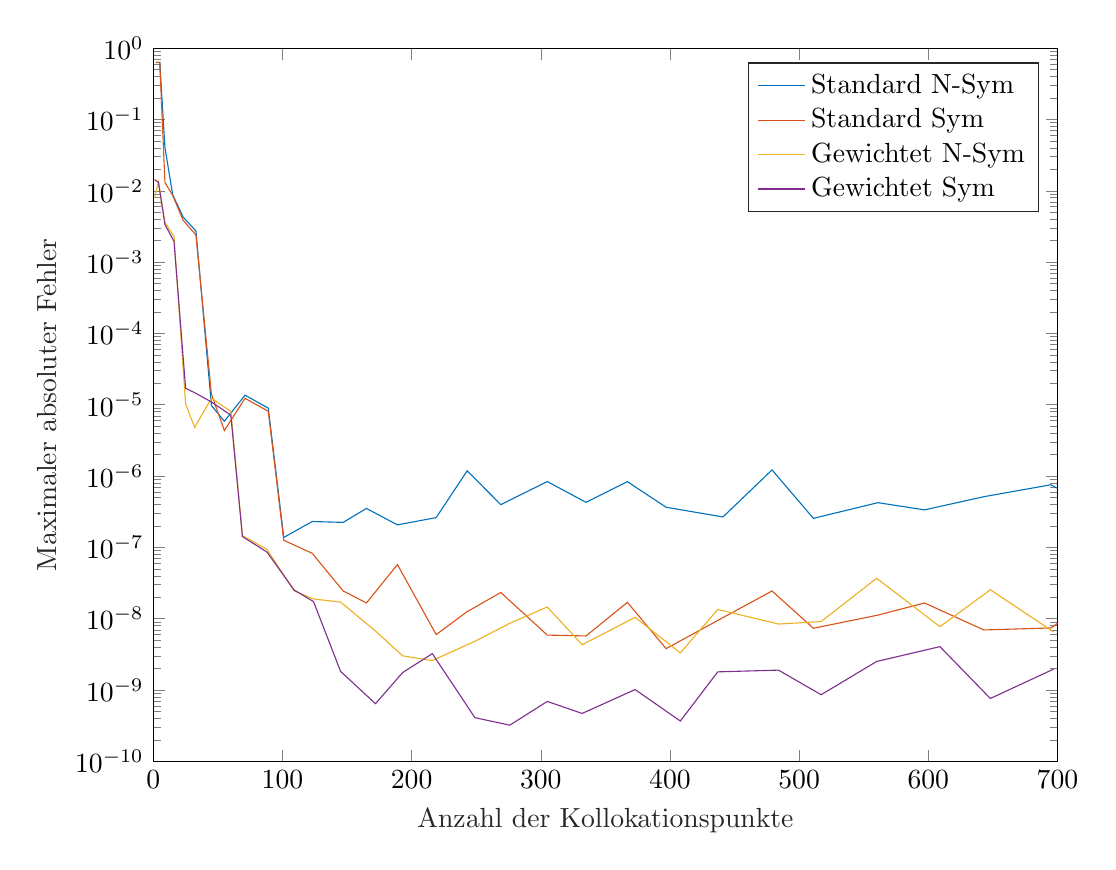
\begin{tikzpicture}

\begin{axis}[%
width=4.521in,
height=3.566in,
at={(0.758in,0.481in)},
scale only axis,
xmin=0,
xmax=700,
xlabel style={font=\color{white!15!black}},
xlabel={Anzahl der Kollokationspunkte},
ymode=log,
ymin=1e-10,
ymax=1,
yminorticks=true,
ylabel style={font=\color{white!15!black}},
ylabel={Maximaler absoluter Fehler},
axis background/.style={fill=white},
%title style={font=\bfseries},
%title={error plot},
legend style={legend cell align=left, align=left, draw=white!15!black}
]
\addplot [color=mycolor1]
  table[row sep=crcr]{%
2	0.631916518837427\\
5	0.631916518837427\\
9	0.0405336006196554\\
15	0.00883209685636366\\
23	0.00430857034180082\\
33	0.00272883525232875\\
45	9.77739763419194e-06\\
55	5.87763883978798e-06\\
71	1.36196952111728e-05\\
89	8.96739386711809e-06\\
101	1.37897394239528e-07\\
123	2.30675160362449e-07\\
147	2.24406043296266e-07\\
165	3.52200691985938e-07\\
189	2.06904876114133e-07\\
219	2.61886160706978e-07\\
243	1.1863207811675e-06\\
269	3.98191725909216e-07\\
305	8.37823561639084e-07\\
335	4.28710712069291e-07\\
367	8.35429125520737e-07\\
397	3.65824390795647e-07\\
441	2.67227388203728e-07\\
479	1.22109189190753e-06\\
511	2.55600133445763e-07\\
561	4.24029023692041e-07\\
597	3.35944663247545e-07\\
643	5.14170673207408e-07\\
695	7.56179082045394e-07\\
737	2.80417328014232e-07\\
789	7.42245731516489e-07\\
};
\addlegendentry{Standard N-Sym}

\addplot [color=mycolor2]
  table[row sep=crcr]{%
2	0.631916518837427\\
5	0.631916518837427\\
9	0.0131196754360414\\
15	0.00861983016720813\\
23	0.00388812001538674\\
33	0.00239333037518191\\
45	1.40699607112382e-05\\
55	4.35500602019578e-06\\
71	1.23129598888494e-05\\
89	8.10392788447301e-06\\
101	1.25844268880626e-07\\
123	8.2670365733617e-08\\
147	2.44909181754127e-08\\
165	1.66449326891027e-08\\
189	5.74401967604748e-08\\
219	5.99240512766386e-09\\
243	1.25718026371124e-08\\
269	2.33486955325546e-08\\
305	5.89867804948185e-09\\
335	5.73415277066447e-09\\
367	1.69623597390256e-08\\
397	3.80944553679541e-09\\
441	1.03664530293202e-08\\
479	2.44956352979386e-08\\
511	7.3530775634989e-09\\
561	1.12447527678139e-08\\
597	1.66316237448783e-08\\
643	6.96026979801756e-09\\
695	7.42834863065589e-09\\
737	2.59786652190286e-08\\
789	6.3033082087216e-09\\
};
\addlegendentry{Standard Sym}

\addplot [color=mycolor3]
  table[row sep=crcr]{%
1	0.00794443935648381\\
4	0.0133017612019765\\
9	0.00362254811444734\\
16	0.0022780437581805\\
25	1.03131710251503e-05\\
32	4.81181204470271e-06\\
45	1.23029704517386e-05\\
60	8.09775474910901e-06\\
69	1.46364200204196e-07\\
88	9.37122425770376e-08\\
109	2.45793275871486e-08\\
124	1.89336762171366e-08\\
145	1.71188485817431e-08\\
172	6.72586053518387e-09\\
193	3.01951863512784e-09\\
216	2.59167542981942e-09\\
249	4.8303522293125e-09\\
276	8.62708293691838e-09\\
305	1.46005317835929e-08\\
332	4.32146185502802e-09\\
373	1.04669000133839e-08\\
408	3.32050553719654e-09\\
437	1.34985452815428e-08\\
484	8.42141356649506e-09\\
517	9.12785619311407e-09\\
560	3.69603436745081e-08\\
609	7.73561570355241e-09\\
648	2.54551856260221e-08\\
697	6.51625686742818e-09\\
};
\addlegendentry{Gewichtet N-Sym}

\addplot [color=mycolor4]
  table[row sep=crcr]{%
1	0.0143846214789116\\
4	0.0130604160741108\\
9	0.00336559573493192\\
16	0.00196288047392809\\
25	1.70127111368545e-05\\
32	1.47805455507494e-05\\
45	1.09439169746484e-05\\
60	7.15540904007439e-06\\
69	1.41731398284328e-07\\
88	8.6057435927378e-08\\
109	2.52869050906823e-08\\
124	1.74264397634349e-08\\
145	1.82477661453406e-09\\
172	6.43924830123765e-10\\
193	1.75784165001858e-09\\
216	3.23772897381502e-09\\
249	4.0984393656629e-10\\
276	3.21971893590955e-10\\
305	6.92943258329137e-10\\
332	4.69699390492906e-10\\
373	1.01659414220023e-09\\
408	3.68062358369059e-10\\
437	1.79956516355162e-09\\
484	1.90341531425275e-09\\
517	8.60199689256547e-10\\
560	2.51715981391953e-09\\
609	4.06107103501085e-09\\
648	7.61975038621188e-10\\
697	1.96490679282846e-09\\
};
\addlegendentry{Gewichtet Sym}

\end{axis}
\end{tikzpicture}%